\subsection{Exemples de Réseaux Neurones à convolution appliqués à l'imagerie RSO}

Dans cette section nous présentons quelques réseaux proposés dans la littératures qui nous semblent des approches intéressantes pour le filtrage des images \acrsar.

\subsubsection{Le filtre  Dn-CNN}

Le réseaux Dn-CNN (\textit{Denoising convolutional neural network}) proposé par Zhang et al. \cite{Zhang2017} permet l'apprentissage intégral d'un filtre de débruitage des images affectées par un bruit additif de type gaussien ($y=x+v$). À la différence des réseaux qui font l'apprentissage d'un modèle directe pour la prédiction de l'image débruitée de la forme $x = F(y)$.  Ce réseau adopte plutôt la modélisation des résidus $R(y) \approx v$, ce qui se traduit par l'équation de prédiction suivante $x=y-R(y)$. L'apprentissage est simplement obtenu par la minimisation de l'erreur quadratique entre les résidus désirés $(y_i-x_i)$ et estimés  $R(y_i)$.  Il en découle la fonction de perte suivante:
\begin{equation}
    l(\Theta)=\frac{1}{2N}\sum_{i=1}^{N}{\parallel R(y_i;\theta) - (y_i-x_i)\parallel}^2
    \label{eq:residual_cost}
\end{equation}
où $\Theta$ représente les paramètres du réseau, $\{(y_i, x_i)\}_{i=1}^{N}$ forme l'ensemble des paires d'image corrompue et propre.

\begin{figure}
  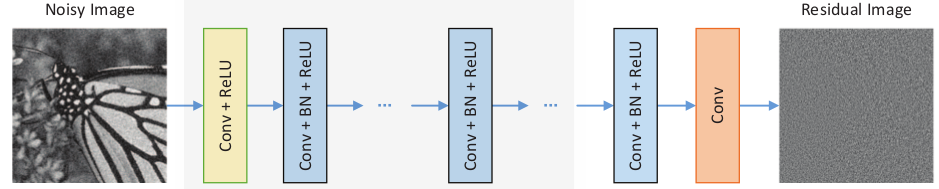
\includegraphics[width=\linewidth]{figures/geo6393/Dn-CNN.png}
   \centering
  \caption{L'architecture du réseau Dn-CNN.}
  \label{fig:DnCNN}
\end{figure}

La Fig. \ref{fig:DnCNN} présente l'architecture du réseau pour réaliser la modélisation des résidus. Le réseau de profondeur $D$ est composé de trois types de blocs de traitement. 1) L'entrée du réseau (\textit{Conv-ReLU}) est formée par une couche de 64 filtres convolutifs de taille $3 \times 3 \times c$, où $c$ est le nombre de canaux d'entrée. Elle génère 64 cartes de caractéristiques qui sont ingérées par une couche d'activation de rectification linéaire (ReLU) pour introduire la non-linéarité. 2) Les couches cachées sont composées par $D-2$ blocs de la forme (\textit{Conv-ReLU-BN}): une couche de 64 filtres convolutifs $3 \times 3 \times 64$, suivi de la fonction non-linéaire ReLU et se finalisant par une couche de normalisation par lot (BN, pour Batch Normalisation) afin d'améliorer et d'accélérer l'apprentissage. Le réseau se termine en sortie par une  couche de $c \times 3 \times 3 \times 64$ filtres qui apprend le résidu pour débruiter l'image.

Deux apprentissages sont effectuées à partir d'échantillons produits à partir de 400 images en ton de gris.  Le premier (Dn-CNN-S) consiste à faire l'apprentissage du réseau sur des niveaux de bruit spécifiés d'avance: $\sigma = $ 15, 25 et 50,  avec une taille de \textit{patch} de $40 \times 40$ et 1600 échantillons pour l'entraînement. Le second (DnCNN-B) est fait à l'aveugle, i.e que le niveau de bruit est aléatoire avec 3000 échantillons. Suite à plusieurs expérimentations, les auteurs proposent une profondeur optimale $D=17$. L'optimisation est faite par l'algorithme du gradient stochastique (SGD, stochastic gradient descent) avec une valeur du \textit{momentum} égale 0.9 et une taille de 128 échantillons par mini-lots. Un \textit{weight decay} égale 0.0001 est appliqué pour pénaliser le surapprentissage. Le paramètre du taux d'apprentissage est fixé à $10^{-1}$ avec une décroissance exponentielle avec une valeur planché de  $10^{-4}$. Le réseau est entraîné sur 50 époques.

\begin{table}
  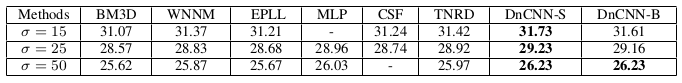
\includegraphics[width=0.9\linewidth]{figures/geo6393/tab_dnCNN.png}
   \centering
  \caption{Résultats comparatifs des deux apprentissages du DnCNN avec des méthodes conventionnelles de pointe. De manière globale, les méthodes par apprentissage profond performent mieux que les méthodes conventionnelles}
  \label{tab:results_DnCNN}
\end{table}

Les résultats des deux apprentissages se comparent favorablement par rapport aux méthodes conventionnelles de pointe comme BMD3, WNNM, EPLL, TNRD.  Les deux réseaux obtiennent des pointages supérieurs en terme de PSNR sur tous les niveaux de bruits testés sur l'ensemble de données BSD68 (voir Tab. \ref{tab:results_DnCNN}).  Sur d'autres ensembles d'images de référence, DnCNN-B se démarque particulièrement pour le niveau de bruit le plus élevé et DnCNN-S pour les autres.  Les auteurs démontrent aussi que l'architecture du réseau s'utilise pareillement pour résoudre d'autres tâches de restauration d'images, comme la supperésolution et le filtrage anti-bloc pour les artéfacts sur les images au format JPEG.

\subsubsection{Le filtre FFDNet}

Le réseaux FFDNet (\textit{Fast and Flexible Denoising Net}) proposé par Zhang et al. \cite{Zhang2018} permet l'apprentissage intégral d'un modèle de débruitage des images affectées par un bruit additif de type gaussien ($y=x+v$). A la différence de la plupart des méthodes qui apprennent un modèle pour un certain niveau de bruit en particulier, FFDNet considère celui-ci comme une variable supplémentaire au modèle, ce qui lui permet une plus grande flexibilité et de mieux généraliser dans les cas de bruits fluctuants dans les images.  Un canal $M$ est ajouté en entrée au réseau avec le niveau de bruit $\sigma$ associé à $y$, $\sigma$ peut être constant ou variable.  L'apprentissage ne se fait pas sur les résidus mais sur le modèle directe  $x = F(y, M)$. De plus, FFDNet travaille sur des sous-images sous-échantillonnées des images originales, réalisant un bon compromis entre la vitesse d'inférence et la performance du débruitage.  L'apprentissage est fait par la minimisation de l'erreur quadratique entre les images désirées $(x)$ et estimées  $F(y_i, M_i)$.  Il en découle la fonction de perte suivante:
\begin{equation}
    l(\Theta)=\frac{1}{2N}\sum_{i=1}^{N}{\parallel F(y_i; M_i;\theta) - x_i\parallel}^2
\end{equation}
où $\Theta$ représente les paramètres du réseau, $\{((y_i,M_i), x_i)\}_{i=1}^{N}$ forme l'ensemble des paires (image cible $+$ image $\sigma"$) et image étiquette.

La Fig. \ref{fig:FDDNet} présente l'architecture du réseau. L'image d'entrée subit une réduction d'échelle d'un facteur 2 et les 4 sous-images décalées sont réorganisées pour former une nouvelle pile de taille  $\frac{W}{2} \times \frac{H}{2} \times 4 \times c$, où $c$ est le nombre de canaux de l'image. À cette pile est enchaînée le canal $M$ représentant le bruit.  Dans le cas d'un bruit blanc gaussien $\sigma$, le canal $M$ est uniforme. Le réseau compte au total $4 \times c + 1$ canaux d'entrée. La partie convolutive de l'architecture est construite de la même manière que celle du DC-CNN.  Après la dernière convolution, les $4 \times c$ sous-images de sortie sont remises à l'échelle originale ($W \times H \times c$) pour former l'images $x$ débruitée. Les auteurs notent qu'il n'y a pas d'avantage à utiliser une architecture résiduelle car le réseau n'est pas assez profond. 

\begin{figure}
  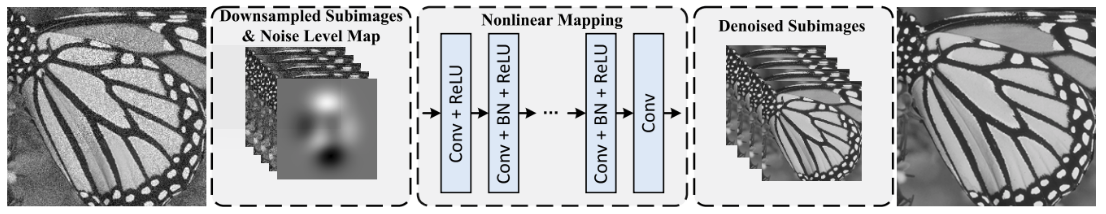
\includegraphics[width=\linewidth]{figures/geo6393/fddnet.png}
   \centering
  \caption{L'architecture du réseau FFDNet.}
  \label{fig:FDDNet}
\end{figure}
\begin{table}
  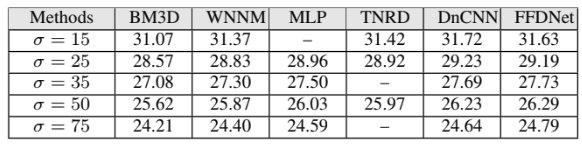
\includegraphics[width=0.6\linewidth]{figures/geo6393/ffdnet_results_bsd68.jpg}
   \centering
  \caption{Résultats comparatifs du FFDNet avec des méthodes conventionnelles de pointe. De manière générale FFDNET surpasse les autres approches pour des niveaux de bruit élevés ou obtient des résultats comparables à DnCNN, avec  lequel il partage une architecture semblable }
  \label{tab:ffdnet_results_bsd68}
\end{table}
L'apprentissage est fait par l'optimiseur ADAM (Kingmam \cite{Kingma2014AdamAM}). L'hyperparamètre du taux d'apprentissage est initialisé à $10^{-3}$ et est réduit à $10^{-4}$ lorsque l'erreur de la régression cesse de diminuer.  Après 5 époques de stagnation, une opération de fusion entre les couches BN et les couches convolutives qui leurs sont ajacentes est appliquée afin de réduire le nombre de paramètres à apprendre et en même temps le taux d'apprentissage est relaxé à $10^{-6}$ pour les 50 dernières époques. 
Les images utilisées pour l'entraînement proviennent de différents ensembles de référence (BSD, ImageNet, Waterloo Exploration Database).  A partir des images en ton gris, des \textit{patch} avec une taille de $50 \times 50$ pixels sont extraites pour former les entrées et un bruit blanc gaussien est ajouté avec un niveau de bruit aléatoire ($\sigma \in [0, 75]$) pour simuler la corruption. Une augmentation des données par des transformations de rotation et de \textit{flip} horizontal et vertical est appliquée pour simuler un plus grand ensemble d'entraînement. 

Les résultats sur l'ensemble de données de référence BSD68 montrent que FFDNET se compare favorablement par rapport aux compétiteurs (BMD3, WNNM, MLP, TNRD et DN-CNN) ou également à DN-CNN.  Il performe mieux que les autres pour des niveaux de bruits élevés ($\sigma \geq 35$) (voir Tab. \ref{tab:ffdnet_results_bsd68}). Une comparaison des temps d'exécution sur CPU (Single Thread) pour le débruitage d'images de tailles différentes démontre que FFDnet est plus rapide que BM3D et nettement plus rapide de DnCNN (voir Fig. \ref{fig:vitesses_ffdnet}).



\begin{figure}
  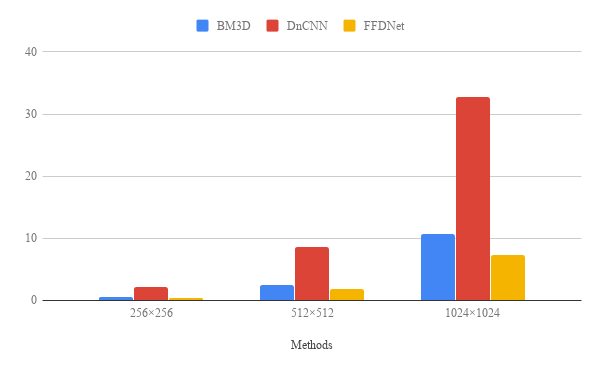
\includegraphics[width=0.75\linewidth]{figures/geo6393/vitesses_ffdnet.png}
   \centering
  \caption{Comparaison des vitesses d'exécution (en secondes) sur CPU (Single Thread).}
  \label{fig:vitesses_ffdnet}
\end{figure}

\subsubsection{Le filtre SAR-CNN}

Sur les traces du DN-CNN, Cherchia et al. \cite{Chierchia2017SARCNN} propose un réseau résiduel SAR-CNN (\textit{SAR Despeckling Convolutional Neural Networks}) pour le filtrage du chatoiement sur les images \acr en intensité. Le réseau est composé de 17 couches convolutives.  Chaque couches calculent 64 cartes de caractéristiques par des convolutions $3 \times 3 \times 64$. La différence fondamentale entre les deux approches est le rejet de la fonction de perte euclidienne, qui selon les auteurs n'est pas adaptée à la statistique du chatoiement.  Le chatoiement est un bruit multiplicatif qui peut être modéliser comme $y=x \cdot v$, où $v$ suit une loi gamma.  L'approche SAR-CNN convertit le bruit multiplicatif en bruit additif par une transformation holomorphique ($ log(y) = log(x \cdot v) = log(x) + w$.  Après la dernière convolution la sortie est reconvertie par l'exponentielle (voir Fig. \ref{fig:SAR-CNN}).  La fonction de perte est adaptée pour tenir compte de la distribution du bruit du chatoiement (par contre l'article n'explique pas très bien l'origine de cette métrique):
\begin{equation}
    l(\Theta)=\sum_{i=1}^{N}{log(cosh(R(y_i;\theta) + c -log \frac{y_i}{x_i}))}
\end{equation}

où $c$ est la valeur positive ($c > 0$) de la moyenne de la distribution logarithmique du chatoiement pour corriger le biais introduit par la transformation holomorphique.

\begin{figure}
  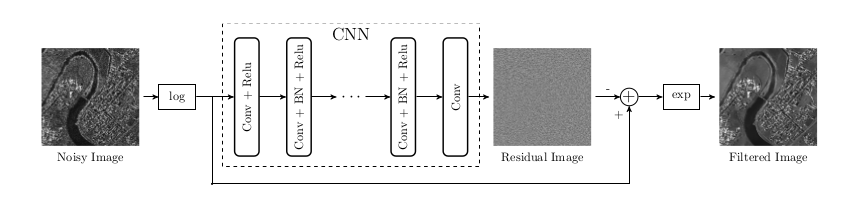
\includegraphics[width=\linewidth]{figures/geo6393/SAR-CNN.png}
   \centering
  \caption{L'architecture du réseau SAR-CNN.}
  \label{fig:SAR-CNN}
\end{figure}

Afin de résoudre le problème symptomatique de l'inexistence de données terrain sans bruit, les auteurs ont synthétisé des échantillons propres sans chatoiement à partir de la moyenne de 26 images \acrsar multi-temporelles coregistrées. Les $2000 \times 128$ paires (propres, bruitées) sont formées par l'extraction de \textit{patch} $40 \times 40$ pixels, à la fois de l'image moyenne et des images bruitées.  L'apprentissage du réseau s'est fait sur 50 époques avec la méthode d'optimisation ADAM et des mini-lots de taille 128.  Le taux d'apprentissage est demeuré fixe sur 30 époques à $10^{-3}$ et abaissé à $10^{-4}$ sur les 20 dernières époques.  La validation durant l'apprentissage est faite à partir des mesures PSNR et SSIM sur des image \acrsar simulées.

Les résultats du SAR-CNN sont comparés avec les 3 techniques de pointe couramment utilisées PPB, NL-SAR, SAR-BM3D. La comparaison est effectuée avec le meilleur modèle SAR-CNN sur des images \acrsar synthétiques.  Comme le démontre le tableau \ref{tab:results-SAR-CNN}, le SAR-CNN obtient de meilleurs résultats à la fois pour la réduction du chatoiement et la conservation des détails.
\begin{table}[h!]
\begin{center}
 \begin{tabular}{||c c c c c||} 
 \hline
  & PPN & NL-SAR & SAR-BM3D & SAR-CNN \\ [0.5ex] 
 \hline
 PSNR moyen & 23.43 & 23.98 & 24.99 & \textbf{25.95} \\
 SIMM moyen & 0.639& 0.677 & 0.729 & \textbf{0.764} \\
 \hline
\end{tabular}
\end{center}
  \caption{Résultats comparatifs du PSNR et du SSIM sur les images \acrsar simulées}
  \label{tab:results-SAR-CNN}
\end{table}

Un autre apprentissage a été effectué à partir d'une pile de 25 images COSMO-SkyMed à une vue. La moitié de la pile a été utilisée pour faire l'entraînement en suivant la procédure décrite auparavant et l'autre moitié a servi à la validation. L'évaluation est faite en mesurant le nombre équivalent de vues (ENL, \textit{equivalent number of looks}) et l'index $\alpha\beta$ (Gomez, \cite{Gomez2016}) qui permet d'évaluer la performance des filtres sur les images \acrsar. SAR-CNN et NL-SAR donnent des résultats similaires en terme de mesure du ENL et de l'index $\alpha\beta$.  Ces deux méthodes déclasses les deux autres facilement (voir \ref{tab:results-SAR-CNN2}). En comparaison avec la première expérimentation faite à partir d'images simulées, l'apprentissage sur des images réelles semble moins performant. La perte semble provenir de la différence entre les images sans bruit et les images bien filtrées qui servent de référence pour l'optimisation du réseau.   

\begin{table}[h!]
\begin{center}
 \begin{tabular}{||c c c c c c||} 
 \hline
 regions & mesure &PPN & NL-SAR & SAR-BM3D & SAR-CNN \\ [0.5ex] 
 \hline
 1 & ENL &47.61 & 154.10& 4.87& 129.10  \\
 2 & ENL &25.28 & 52.12 & 4.71 & 56.32 \\
 \hline
  1 & $\alpha\beta$ &0.162& 0.076& 0.530& 0.187 \\
 2 & $\alpha\beta$ &0.171&0.065& 0.511& 0.182 \\
  \hline
\end{tabular}
\end{center}
  \caption{Résultats comparatifs du ENL et de l'index $\alpha\beta$ sur les images \acrsar réelles}
  \label{tab:results-SAR-CNN2}
\end{table}

\subsubsection{Le filtre ID-CNN}

Comme ces compatriotes précédents, le filtre ID-CNN (\textit{Image Despeckling Convolutional Neural Network}) proposé par Wang et al. \cite{Wang2017IDCNN} modélise les résidus afin de réduire le chatoiement des images \acrsar. Cependant, il n'applique pas de transformation holomorphique au signal d'entrée mais estime directement le chatoiement en utilisant le modèle du bruit multiplicatif ($y=x \cdot v$). Assez inusité, l'opération résiduelle utilise la division pour calculer la valeur des résidus en divisant l'image d'entrée par l'estimation du chatoiement apprise par le réseau. Celui-ci est formé de 8 couches du même type que celles de l'architecture Dn-CNN.  Avec seulement 8 couches, ce réseau est nettement moins profond que les autres (voir Fig. \ref{fig:ID-CNN}). Le Tab. \ref{tab:conf-ID-CNN} présente les détails de la configuration du réseau.

\begin{figure}
  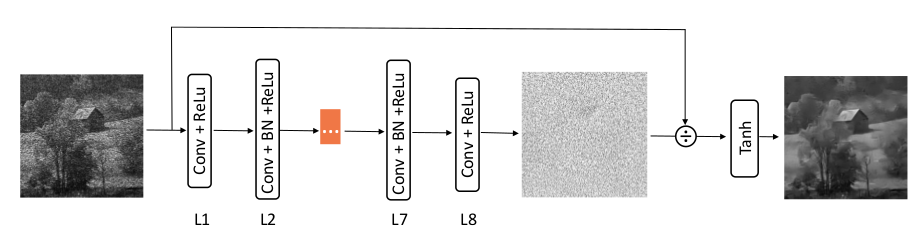
\includegraphics[width=\linewidth]{figures/geo6393/id-cnn.png}
   \centering
  \caption{L'architecture du réseau ID-CNN.}
  \label{fig:ID-CNN}
\end{figure}

\begin{table}[h!]
\begin{center}
 \begin{tabular}{||c c c c||} 
 \hline
  & couche & taille du filtre & nombre de filtre  \\ [0.5ex] 
 \hline
L1 & \text{Conv-ReLU} & $3 \times 3 \times$ 1 & 64  \\
L2-L7 & \text{Conv-BN-ReLU} & $3 \times 3 \times1$  & 64   \\
L8 & \text{Conv-ReLU} & $3 \times 3 \times$ 1 & 1  \\
  \hline
\end{tabular}
\end{center}
  \caption{Configuration du réseau ID-CNN}
  \label{tab:conf-ID-CNN}
\end{table}

\begin{table}
  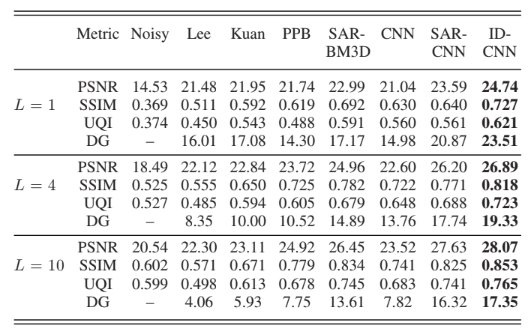
\includegraphics[width=0.6\linewidth]{figures/geo6393/id-cnn-resultats.jpg}
   \centering
  \caption{Résultats comparatifs de ID-CNN avec des méthodes traditionnelles en radar (Lee, Kuan) et conventionnelles de pointe (PPB, SAR-BM3D) et des approches en apprentissage machine profond (CNN=Dn-CNN, SAR-CNN. }.
  \label{tab:id-cnn-resultats}
\end{table}

L'apprentissage du réseau est fait en minimisant une composition de fonctions de pertes:
\begin{equation}
    l(\Theta)_{total} = l(\Theta)_E + \lambda_{TV} \cdot l(\Theta)_{TV}
\end{equation}
où $ l(\Theta)_E $ représente la fonction de perte euclidienne:
\begin{equation}
    l(\Theta)=\frac{1}{2N}\sum_{i=1}^{N}{\parallel R(y_i;\Theta) - (y_i-x_i)\parallel}^2
\end{equation}
où $\Theta$ correspond aux paramètres du réseau, $\{(y_i, x_i)\}_{i=1}^{N}$ forme l'ensemble des paires d'image cibles et étiquettes et $l(\Theta)_{TV}$ est la fonction de perte qui calcule la variation totale :
\begin{equation}
    l_{TV}(\Theta)=\sum_{w=1}^{W} \sum_{h=1}^{H} \sqrt{((X^{w+1, h}-X^{w, h})^2 + (X^{w, h+1}-X^{w, h})^2)}
\end{equation}
où $w$ et $h$ sont les index des pixels d'une image $W \times H$ et X représente la valeur du pixel. Selon les auteurs, la fonction de perte euclidienne est responsable du filtrage du chatoiement tandis que la fonction de perte de la variation totale est responsable du lissage.  Le paramètre $\lambda_{TV}$ pondère l'intensité du lissage.  Ce paramètre est fixé à une valeur plus petite que 1 afin de ne pas perdre trop de détails au dépend du lissage. Le réseau est entraîné sur 3580 images de taille $256 \times 256$ avec un bruit multiplicatif simulé en fonction du nombre de vues ($L$).  L'apprentissage des paramètres est calculé par l'optimiseur ADAM, avec des mini-lots de 16 et un taux d'apprentissage fixé à 0.0002. Le paramètre $\lambda_{TV}$ est fixe à 0.002.  Trois apprentissages ont été effectués en fonction du nombre de vues $(L=1, L=4, L=10)$ et les performances ont été calculées sur 85 images indépendantes de l'ensemble d'entraînement.

L'évaluation de la performance est calculée à partir des 4 métriques suivantes: PSNR, SSIM, l'index de qualité universel (UQI) et le gain de suppression du chatoiement (DG, \textit{despeckling gain}). Les résultats obtenus sont étonnements bons.  ID-CNN  obtient les meilleurs scores toutes catégories de mesures confondues.  De plus, grâce au fait que l'architecture soit peu profonde, la vitesse d'exécution sur gpu (0.56 sec.) est environ 5 fois plus rapide que son plus proche compétiteur Dn-CNN (2.42 sec.). Malheureusement les auteurs ne donnent pas d'explications satisfaisantes sur le choix de leur architecture et de la fonction de perte. A noter que Dn-CNN correspond à l'approche CNN dans l'article.

\subsubsection{Le filtre SAR-DRN}

Les auteurs (Zhang et al. \cite{Zhang2018LearningSAR-DRN}, un autre que ceux des articles précédents) propose un filtre SAR-DRN (\textit {SAR Dilated Residus Network}) qui s'entraîne bout en bout avec des convolution dilatées (ou à trou).  Ces convolutions ont un paramètre appelé le niveau de dilatation qui définit l'espace entre les éléments du filtre convolutif. Augmenter le niveau de dilatation permet d'augmenter le champs réceptif du ConvNet sans augmenter le nombre de paramètres. Élargir le champs réceptif permet à son tour de capturer plus de contexte  autour d'un point et possiblement améliorer la capacité discriminatoire du réseau.  Le réseau est composé de 7 couches de convolutions dilatées plus deux sauts de connections (voir Fig. \ref{fig:SAR-DRN}).  L'ajout des sauts de connections aide à la convergence de l'apprentissage. Celui-ci se fait sans utiliser de transformation logarithmique (SAR-CNN) et sans modification de la fonction de perte (ID-CNN).  La dilatation des convolutions suit le schème telle que décrit par le Tab .\ref{tab:conf-SAR-DRN}.  L'apprentissage suit le même procédé que dans le cas de Dn-CNN avec la minimisation de la fonction de perte euclidienne sur les résidus (voir \ref{eq:residual_cost}).  L'optimiseur utilisé est toujours ADAM et le taux d'apprentissage est initialisé à 0.01 et est diminué à toute les 10 époques sur 50. Plusieurs modèles ont été entraînés pour les quatre niveaux de bruit radar (L=1, 2, 4 et 8).

\begin{figure}
  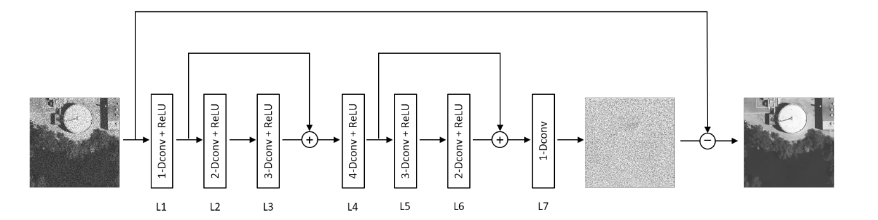
\includegraphics[width=\linewidth]{figures/geo6393/SAR-DRN.png}
   \centering
  \caption{L'architecture du réseau SAR-DRN}
  \label{fig:SAR-DRN}
\end{figure}


\begin{table}[h!]
\begin{center}
 \begin{tabular}{||c c c c c||} 
 \hline
couche & niveau de dilatation & bloc & padding des convolutions & filtres \\ [0.5ex] 
 \hline
L1 & 1 & 1 & Convolution Dilatée + ReLU & $64 \times 3 \times 3$\\
L2 & 2 & 2 & Convolution Dilatée + ReLU  &$64 \times 3 \times 3$    \\
L3 & 3 & 3 & Convolution Dilatée + ReLU & $64 \times 3 \times 3$    \\
L4 & 4 & 4 & Convolution Dilatée + ReLU & $64 \times 3 \times 3$    \\
L5 & 3 & 3 & Convolution Dilatée + ReLU & $64 \times 3 \times 3$    \\
L6 & 2 & 2 & Convolution Dilatée + ReLU & $64 \times 3 \times 3$    \\
L7 & 1 & 1 & Convolution Dilatée  & $64 \times 3 \times 3$    \\
  \hline
\end{tabular}
\end{center}
  \caption{Description de réseau SAR-DRN}
  \label{tab:conf-SAR-DRN}
\end{table}

Afin de tester leur algorithme, les auteurs ont sélectionné les 4 approches suivantes: PPB, SAR-BM3D, SAR-POTDF et SAR-CNN. L'évaluation de la performance est calculée à partir des 2 métriques suivantes: PSNR, SSIM sur trois images provenant de différents milieux.  

\subsection{Exemples de Réseaux Neurones à convolution appliqués à l'imagerie \acrpolsar}

\begin{figure}
  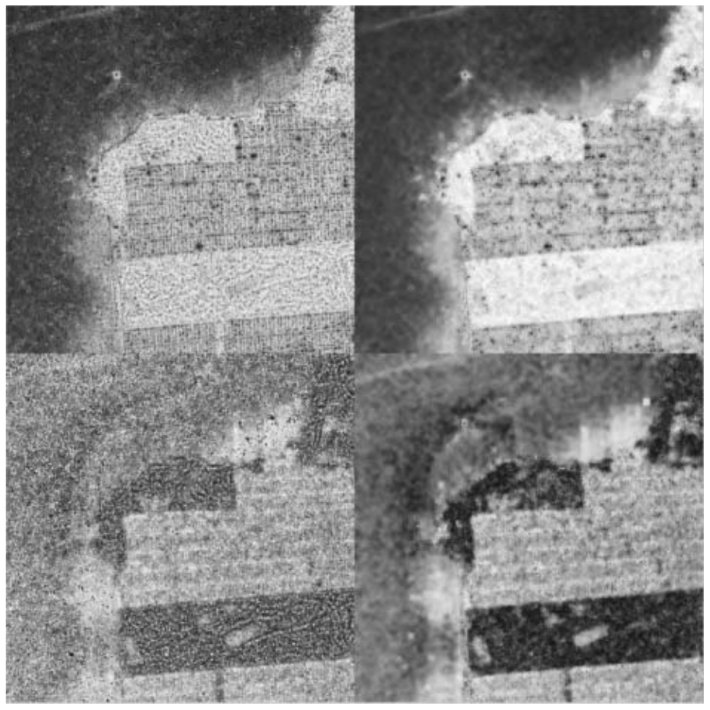
\includegraphics[width=0.5\linewidth]{figures/geo6393/test-foucher2017.jpg}
   \centering
  \caption{L'entropie (rangée supérieure) et l'anisotropie (rangée inférieure) pour un filtre de Lee $7 \times 7$ et pour l'approche de (Foucher et al. \cite{Foucher2017})}
  \label{fig:foucher2017}
\end{figure}

La littérature sur le filtrage des images polarimétriques à l'aide de réseaux à convolution est plus rare.  Nous ne présentons que quelques exemples. 

Quelques articles semblent directement s'intéresser à la question (Foucher et al. \cite{Foucher2017}).  Les auteurs explorent en particulier l'impact du filtrage sur les mesures polarimétriques de la décomposition H-A-Alpha. L'apprentissage du modèle est calculé sur les valeurs du \textbf{span} de la matrice de cohérence $\begin{bmatrix} T_3 \end{bmatrix}$ sur des données simulées 1 look.  Le réseau entraîné est adapté de l'architecture de (Dong, \cite{Dong2016}) utilisé en super-résolution. Le modèle est par la suite employé dans un filtre itératif. Les tests sur l'image AIRSAR de San-Francisco avec une décomposition polarimétrique de Cloud-Pottier sont encourageants. Ils montrent une bonne préservation des paramètres tout en filtrant le chatoiement et sans perdre trop de détails (voir Fig. \ref{fig:foucher2017}).  Les auteurs concluent que malgré de bon résultats, le choix d'une bonne architecture neuronale pour le filtrage polarimétrique demeure un problème ouvert.  De plus la préservation des cibles ponctuelles posent toujours un problème à cause de l'aspect convolutionnel du réseaux.  Ce qui soulève d'autres questions du  point de vue de l'ensemble de données pour l'apprentissage et de sa représentativité du point de vue polarimétrique.

 Par contre, on retrouve certaines études en classifications polarimétriques qui indirectement font du filtrage.  Les auteurs Li et all \cite{Li2018Classification} proposent un réseau de type FCN pour la classification des images polarimétriques basé sur les paramètres de Cloud-Pottier.  La matrices de covariance $\begin{bmatrix} T_3 \end{bmatrix}$ est fournie en entrée du réseau pour estimer les  paramètres ($H, A, \bar \alpha, \lambda_1,  \lambda_2  \lambda_3$).  Le filtrage est indirecte dans le sens que pour obtenir des valeurs débruitées en sortie, le réseau a appris comment filtrer le chatoiement.  Un véritable filtrage serait d'estimer la matrice  $\begin{bmatrix} T_3 \end{bmatrix}$ débruitée directement.


\section{Conclusion}

Nous avons présenté un survol de la théorie de la polarimétrie appliquée aux images satellites \acrpolsar ainsi qu'un les grandes lignes de l'apprentissage machine profond et l'utilisation des \acrconvnet pour l'analyse des images. Avec ces connaissances nous pouvons entreprendre la mise en place des différents aspects des expérimentations et tests que nous voulons effectuer.